\documentclass{beamer}

\mode<presentation> {
\usetheme{Madrid}
}

\usepackage{graphicx} % Allows including images
\usepackage{booktabs} % Allows the use of \toprule, \midrule and \bottomrule in tables

%----------------------------------------------------------------------------------------
%	TITLE PAGE
%----------------------------------------------------------------------------------------

\title[Clustering Project]{Clustering and Distance Methods} % The short title appears at the bottom of every slide, the full title is only on the title page

\author{Justin Hood} % Your name
\institute[UW-Stout] % Your institution as it will appear on the bottom of every slide, may be shorthand to save space
{
University of Wisconsin-Stout \\ % Your institution for the title page
\medskip
\textit{hoodj5402@uwstout.edu} % Your email address
}
\date{\today} % Date, can be changed to a custom date

\begin{document}

\begin{frame}
\titlepage % Print the title page as the first slide
\end{frame}

\begin{frame}
\frametitle{Outline} % Table of contents slide, comment this block out to remove it
\tableofcontents % Throughout your presentation, if you choose to use \section{} and \subsection{} commands, these will automatically be printed on this slide as an overview of your presentation
\end{frame}

%----------------------------------------------------------------------------------------
%	PRESENTATION SLIDES
%----------------------------------------------------------------------------------------

%------------------------------------------------
\section{Introduction} % Sections can be created in order to organize your presentation into discrete blocks, all sections and subsections are automatically printed in the table of contents as an overview of the talk
%------------------------------------------------

%\subsection{Subsection Example} % A subsection can be created just before a set of slides with a common theme to further break down your presentation into chunks

\begin{frame}
\frametitle{Background}
\begin{itemize}
\item Over the course of studying statistics at any level, it becomes natural to consider data that is categorical in nature.
\pause
\item Oftentimes multivariate data exhibits a natrual grouping or clustering behavior that is challenging to analytically describe.
\pause
\item The goal of clustering analysis is to find the natural groupings that exist within the data without requiring assumptions by the statistician.
\end{itemize}
\end{frame}

\begin{frame}
\frametitle{Cluster vs. Classification}
\begin{itemize}
\item Classification is another tool that statisticians can use to group data structures together.
\pause
\item It requires that the statistician choose a number of groupings before analysis. This can be problematic on large data sets as well as on data whose shape is not well known before.
\pause
\item Clustering is a more base and general process that allows the data to naturally sift into groupings based on the user defined ``distance". We will focus on this method for this project.
\end{itemize}
\end{frame}

\begin{frame}
\frametitle{What is Distance?}
\begin{itemize}
\item Topologically speaking, we can think about clustering as wrapping $n$-dimensional hyperspheres around the data in $n$-dimensional space, where our goal is to find the most natural centers and radii that cover the data.\\
\pause
For a 2-D example, consider the image below,
\begin{center}
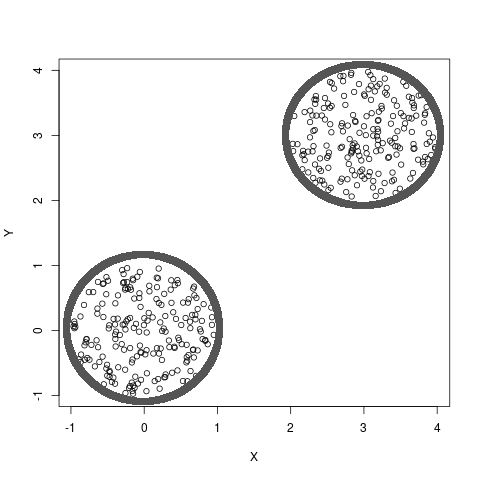
\includegraphics[scale=.20]{circles.png}
\end{center}
\item We see that these two clusters of points have natural circular boundaries.
\end{itemize}
\end{frame}
\begin{frame}
\frametitle{Distance Continued}
\begin{itemize}
\item For high dimensions and categorical data, distance is harder to visualize, but the rough idea is the same.
\pause
\item The problem is defining a meaningful metric to compare points.
\end{itemize}
\end{frame}

\begin{frame}
\frametitle{Common Measures of Distance}
\begin{itemize}
\item Euclidean distance: $d(x,y)=\sqrt{\sum_i (x_i-y_i)^2}$
\item Minkowski Metric (Taxicab distance), $d(x,y)=\left[\sum_{i=1}^p|x_i-y_i|^m\right]^{1/m}$
\item Canberra metric $d(x,y)=\sum_i \frac{|x_i-y_i|}{x_i+y_i}$
\pause
\item Other examples include hamming distance and the ``max metric"
\end{itemize}
\end{frame}

\section{Comparing Data}
\begin{frame}
\frametitle{Similarity Coefficient}
\begin{itemize}
\item For characteristic data, it is often helpful to introduce a binary variable for the purposes of comparison.\\
\pause
For example, consider the data below,
\begin{center}
\begin{tabular}{c|ccccc}
& 1 & 2 & 3 & 4 & 5\\\hline
$i$ & 1 & 0 & 0 & 1 & 1\\
$k$ & 1 & 1 & 0 & 1 & 0
\end{tabular}
\end{center}
\pause
We may then write,
\[d(i,k)=\begin{cases}
0 & i=k\\
1 & i\neq k
\end{cases}\]\pause
So, $d$ is a measurement of ``difference" in the two variables
\end{itemize}
\end{frame}
\begin{frame}
\frametitle{Similarity Coefficient Continued}
In this way, we can write the comparisons in the table,
\begin{center}
\begin{tabular}{c|cc|c}
& $k=1$ & $k=0$ & Totals\\\hline
$i=1$ & $a$ & $b$ & $a+b$\\
$i=0$ & $c$ & $d$ & $c+d$\\\hline
Totals & $a+c$ & $b+d$ & $a+b+c+d$
\end{tabular}
\end{center}
\pause
From this table, we can define many similarity coefficients depending on our desired measurement. These coefficients are then collected into matrices, upon which we can perform our more familiar statistical operations.
\end{frame}
\begin{frame}
\frametitle{Methods}
\begin{itemize}
\item Now that we have considered how we might compare our abstract data, let us now consider how we will go about sorting it.
\pause
\item We will first consider hierarchical clustering methods, which have two types,
\pause
\begin{itemize}
\item Agglomerative (Start with $n$ clusters and combine)\\
\item Divisive (Start with $1$ cluster and partition)
\end{itemize}
\end{itemize}
\end{frame}
\begin{frame}
\frametitle{Agglomerative Method Steps}
For an agglomerative method, the basic steps are,
\begin{enumerate}
\item Start with $n$ clusters, and an $n\times n$ matrix of distance values.
\pause
\item Find the entry or entries with the lowest distance value.
\pause
\item Merge these pairs of clusters, and update the matrix by removing the old entries and recalculating distances relative to the new merged groups.
\pause
\item Rinse and repeat $n-1$ times. Keep a record of each merge as it happens for plotting purposes.
\end{enumerate}
\end{frame}

\begin{frame}
\frametitle{Dendrogram Example}
Using the agglomerative method on Concordance data from several different languages, we arrive at,\\
\begin{columns}
\column{0.75\textwidth}
\begin{figure}[ht]
\begin{center}
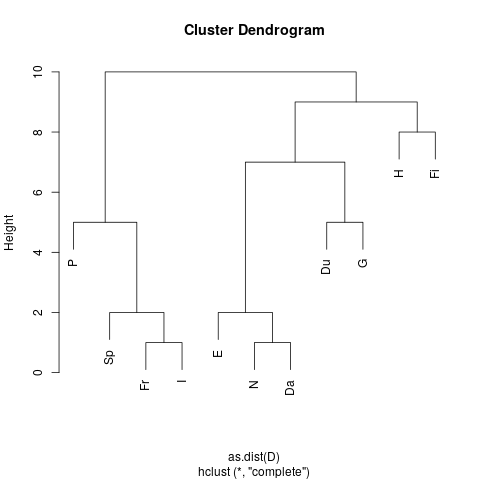
\includegraphics[scale=.45]{LanguageDendo.png}
\end{center}
\end{figure}
\column{0.25\textwidth} 
 This result shows that French and Itailian are closely related, and that Danish and Norwegian are as well. To the French and Italian, we see that Spanish is also closely related, and so on.
\end{columns}
\end{frame}

\begin{frame}
\frametitle{Hierarchical Methods}
When we compute the steps of these agglomerative methods, we must consider the different ways we can join the subgroups.
\begin{itemize}
\item Single Linkage - Find the smallest values in the distance matrix and join those groups together
\item Complete Linkage - Much the same as the former, however our updated matrix uses the maximum distance between the subgroups when updating
\item Average Linkage - Updating the matrix uses the average of all possible distances from the original grouping.
\item Wards Method - Seeks to minimize ESS. Treats each cluster as an n-sphere and computes the distance to the centroid. Each succesive merger results in the smallest possible ESS based on these centers and groupings.
\end{itemize}
\end{frame}

\begin{frame}
\frametitle{Hierarchical Continued}
\begin{itemize}
\item As we see, there are many different ways to compute the iterative steps of these hierarchical methods.
\pause
\item Due to the nature of the methods, we have no statistically sound way of identifying and cleaning outliers from the data, which can result in bad clustering.
\pause
\item There is also no way to change a points assignment once it has been merged into a new cluster. As such, points can be grouped incorrectly.
\pause
\item Using multiple different methods and comparing the results is often the best way to decide if your results are stable and correct.
\end{itemize}
\end{frame}

\section{Non Hierarchical Methods}
\begin{frame}
\frametitle{Nonhierarchical Methods}
\begin{itemize}
\item We saw before that Hierarchical methods are designed to group variables into groups.
\item We now consider methods that group items into an arbitrary number of groups by recursively updating.
\item This is commonly done by choosing ``seed" points at random within the space of the data.
\end{itemize}
\end{frame}

\begin{frame}
\frametitle{K-means Method}
We now consider a popular nonhierarchical method, K-means. The steps of this method are,
\pause
\begin{enumerate}
\item Partition the points into $K$ initial clusters
\pause
\item Iteratively compute the distances to the centroids of each cluster for each data point, and move the point to a better cluster if necessary.
\pause
\item Update the affected centroids
\pause
\item Rinse and Repeat until each point is in the best possible centroid for itself
\end{enumerate}
\end{frame}

\begin{frame}
\frametitle{K-means Example}
\begin{columns}
\column{0.5\textwidth}
Consider the data,
\begin{tabular}{c|cc}
Item & $x_1$ & $x_2$\\\hline
A & 5 & 3\\
B & -1 & 1\\
C & 1 & -2\\
D & -3 & -2
\end{tabular}\\
To perform a K-means clustering, let us at random choose an initial partition of $(AB)$ and $(CD)$. We find the centroid of each of these to be,
\begin{tabular}{c|cc}
Cluster & $x_1$ & $x_2$\\\hline
(AB) & $\frac{5-1}{2}=2$ & $\frac{3+1}{2}=2$\\
(CD) & $\frac{1-3}{2}=-1$ & $\frac{-2-2}{2}=-2$
\end{tabular}\\
So, we have our centroids, $(2,2)$ and $(-1,-2)$. Next, we compute the distances between each point and the centroids,
\column{0.5\textwidth}
\begin{align*}
d(A,(AB)) &= \sqrt{10}\\
d(A,(CD)) &= \sqrt{61}\\
d(B,(AB)) &= \sqrt{10}\\
d(B,(CD)) &= \sqrt{9}
\end{align*}
Here, we see that $B$ is actually closer to the centroid of $(CD)$, and as such, we shall move it, and update the centroids. Continuing,
\begin{align*}
d(C,(A)) &= \sqrt{41}\\
d(C,(BCD)) &= \sqrt{5}\\
d(D,(A)) &= \sqrt{89}\\
d(D,(BCD)) &= \sqrt{5}
\end{align*}
\end{columns}
\end{frame}

\begin{frame}
\frametitle{K-means Continued}
\begin{itemize}
\item We see now that none of the points need to be moved, and as such, we are done with our calculations.
\item The resulting groups $(A)$ and $(BCD)$ make sense upon inspection, as $BCD$ all lie at least partly within the negative ranges around the origin, while $A$ sits alone in quadrant I with a ways between it and the other points.
\item As before, it is recommended to re-run the algorithm with different initial conditions, to test stability.
\end{itemize}
\end{frame}

\begin{frame}
\frametitle{NonHierarchical Method Notes}
\begin{itemize}
\item It is important to make sure that our initial conditions do not inadvertently overlap.
\pause
\item Outliers will tend to isolate themselves into their own groups.
\pause
\item Even if you know the number of groups a population has, if the sampling method does not have points in each cluster, a forced number of clusters might have bad results.
\end{itemize}
\end{frame}

\section{Clustering Based on Statistical Models}
\begin{frame}
\frametitle{Clustering Based on Statistical Models}
\begin{itemize}
\item The methods that we have considered before have all been fairly intuitive in terms of the derivation of the steps, but there exist more statistically model based methods for analyzing the data.
\item For example, consider the model where each cluster $k$ has an expected proportion $p_k$ of the points, and the associated pdf $f_k(x)$. Then, for $k$ clusters,
\[f_{Mix}(x)=\sum p_kf_k(x)\]
\item As one might expect, a common mixture model is a multivariate normal distribution.
\end{itemize}
\end{frame}

\begin{frame}
\frametitle{Further Analysis of the Normal Model}
\begin{itemize}
\item As one might expect, this normal distribution model will yield results close to the K-means and Ward's method processes.
\item Choosing the number of clusters for an arbitrary data set can be challenging, but the formula
\[\#Clusters \propto -2\ln(L_{max})-Penalty\]
where $L_{max}$ is defined as the product of our mixture functions.
\item Under the AIC the penalty can be written as,
\[-2\ln(L_{max})-2N(\frac{k}{2}(p+1)(p+2)-1)\]
\end{itemize}
\end{frame}

\begin{frame}
\frametitle{Multidimensional Scaling}
\begin{itemize}
\item As one might expect, a natural consequence of looking at these high dimensional abstract data sets will be to attempt to project them into a lower dimensional form for graphical interpretation.
\item This, however will not always be a simple procedure, as information is lost through the projection into lower dimensions, as well as the fact that trying to encode categorical data always results in loss of precision as well.
\item As such, we might consider a process similar to PCA to attempt to look at the data while retaining as much information as possible.
\item Multidimensional scaling looks at a slightly different problem than PCA, however, as the relative distances between the points should be retained when possible, as this can provide interesting analytical results on high dimensional data.
\end{itemize}
\end{frame}

\begin{frame}
\frametitle{Multidimensional Scaling Continued}
\begin{itemize}
\item Looking at $N$ observations, there are $M=N(N-1)/2$ similarities between points. Assuming the data is fine enough that equal values are not possible, it is trivially possible to order these distances,
\[s_{1} < s_{2} <\ldots < s_{M}\]
As such we would expect that the associated distances to follow the form,
\[d_1^q > d_2^q > \ldots > d_M^q\]
Where $q$ is the desired dimensionality of the projection.
\item For cases when a the transformation from $s$ to $d$ is not as simple, a computation of the Stress is used to align the data accordingly.
\item An interesting consequence of this analysis is that on data about physical distances, the resultant plot will artificially start to resemble a map without the data ever being placed in that shape.
\end{itemize}
\end{frame}

\begin{frame}
\frametitle{Correspondence Analysis}
\begin{itemize}
\item Another way of graphically representing complex higher dimensional data is Corresponednce analysis.
\item This method is used for frequency data.
\item By representing relative frequency in the form of stacked bar charts, both the categories and the levels can be compared simultaneously.
\end{itemize}
\end{frame}

\begin{frame}
\frametitle{Correspondence Analysis Numerics}
\begin{itemize}
\item To 
\end{itemize}
\end{frame}
\end{document} 